
%(BEGIN_QUESTION)
% Copyright 2010, Tony R. Kuphaldt, released under the Creative Commons Attribution License (v 1.0)
% This means you may do almost anything with this work of mine, so long as you give me proper credit

An antimicrobial agent called {\it acrolein} used to protect diesel fuel from fungal growth may be manufactured by reacting propylene with steam and air in a reactor vessel.  The ensuing chemical reaction is exothermic, and so a coolant loop using a special heat-transfer oil called ``Dowtherm'' is used to remove heat from the reactor vessel.  Suppose operators call you to troubleshoot a process problem they are having, and show you this graphic display on their control system monitor:

$$\includegraphics[width=15.5cm]{i00365x01.eps}$$

The reactor (R-23) is operating at much too high a temperature.  Even the temperature controller TC-99 shows the reactor outlet temperature well above setpoint.  The operator further tells you that he is accustomed to seeing the Dowtherm pump discharge temperature be a lot lower: more like 260 $^{o}$F instead of 322 $^{o}$F.  He furthermore tells you he is accustomed to seeing the water discharge from E-77 to the cooling tower at a much greater temperature than 90 $^{o}$F.

\vskip 10pt

Based on the information found in this graphic display, help the operator identify the most likely cause of the overheated reactor (from the list below), and explain why you chose the answer you did:

\begin{itemize}
\item{} Control valve TV-101 mechanically stuck wide open
\item{} Water cooling tower turned off (not cooling water enough)
\item{} Heat exchanger E-61 poor heat transfer because of ``fouling'' on tubes
\item{} Control valve TV-99 mechanically stuck open
\item{} Heat exchanger E-77 poor heat transfer because of ``fouling'' on tubes
\item{} Control valve TV-99 mechanically stuck closed
\item{} Controller TC-99 left in manual mode
\item{} Dowtherm pump running too fast (flow too great)
\end{itemize}

\filbreak


\underbar{file i00365}
%(END_QUESTION)





%(BEGIN_ANSWER)

{\bf Heat exchanger E-77 poor heat transfer because of ``fouling'' on tubes} is the most likely of the given causes, because it explains why the Dowtherm discharge temperature is too high and also why the cooling water discharge temperature from that exchanger isn't very high compared with the cooling water inlet temperature.

Control valve TV-99 sticking closed would also explain the high Dowtherm temperature, because it would cause all the cooling water to boil out of the exchanger (E-77), eventually leaving no flow through the outgoing line.  This would allow it to cool and possibly read 90 degrees as it is doing now.

\vskip 10pt

5 points for correct choice, 5 points for logical explanation.

%(END_ANSWER)





%(BEGIN_NOTES)

{\bf This question is intended for exams only and not worksheets!}.

%INDEX% Process: acrolein production 

%(END_NOTES)

